\documentclass[dvipsnames,11pt]{article}
\usepackage{amsmath}

%Hey, if you're using this preamble it means that it was probably written by Stefano Graziosi (me). If you see something that doesn't make sense, feel free to email me at stefano.graziosi@studbocconi.it
%p.s. in case it's not already evident from the preamble, I'm not a professional LaTeX user, so I'm sure there are better ways to do things. I'm just trying to make it work.

%------------------------------------------------------------------------------
%           LAST UPDATE: 30-01-2025
%------------------------------------------------------------------------------

%I don't own copyright on anything, I just literally copied and pasted together a bunch of stuff.

%Credit goes to the original authors.

%------------------------------------------------------------------------------
%           Packages
%------------------------------------------------------------------------------

\usepackage{fancyhdr}
\usepackage[dvipsnames]{xcolor}
\usepackage[many]{tcolorbox}
\usepackage[all]{xy}
\usepackage{tcolorbox}
\usepackage{graphicx}
\usepackage{hyperref}
\usepackage{xcolor}    
\usepackage{wrapfig}
\usepackage{amsmath, amssymb, amsthm}
\usepackage{titlesec}
\usepackage{halloweenmath}
\usepackage{enumitem}
\usepackage{listings}
\usepackage{kantlipsum}
\usepackage{pdfpages}

\usepackage[T1]{fontenc}                            % Font Styling
\usepackage{lmodern,mathrsfs}


\usepackage{mathtools,amsthm,amssymb,amsfonts,bm}   % Math Presets
\usepackage{thmtools,amsmath}
\usepackage{array,tabularx,booktabs}                % Table Presets
\usepackage{graphicx,wrapfig,float,caption}         % Figure Presets
\usepackage{setspace,multicol}                      % Text Presets
\usepackage{tikz,physics}                           % Physics Presets

\usepackage{titlepic}
\usepackage{pdfpages}

%------------------------------------------------------------------------------
%           Geometry
%------------------------------------------------------------------------------

\usepackage[a4paper,margin=1in]{geometry}
%\usepackage[margin=1in]{geometry}

%------------------------------------------------------------------------------
%           Chapter and section formatting
%------------------------------------------------------------------------------

%\renewcommand{\chaptername}{Lecture}
%\renewcommand\thesection{P~\arabic{section}}

\renewcommand{\thefigure}{\thesection-\arabic{figure}}
\renewcommand{\thetable}{\thesection-\arabic{table}}

%------------------------------------------------------------------------------
%           Colours
%------------------------------------------------------------------------------

\definecolor{sgblue}{rgb}{0, 169, 211}
\definecolor{sggreen}{rgb}{0, 164, 0}
\definecolor{sgpurple}{rgb}{99, 0, 165}
\definecolor{sgyellow}{rgb}{255, 211, 0}
\definecolor{sgorange}{rgb}{255, 127, 20}

\definecolor{sbblue}{rgb}{219, 248, 254}
\definecolor{sbgreen}{rgb}{223, 255, 218}
\definecolor{sbpurple}{rgb}{241, 220, 255}

\definecolor{codegreen}{rgb}{0,0.6,0}
\definecolor{codegray}{rgb}{0.5,0.5,0.5}
\definecolor{codepurple}{rgb}{0.58,0,0.82}
\definecolor{backcolour}{rgb}{0.95,0.95,0.92}

%------------------------------------------------------------------------------
%           Environments
%------------------------------------------------------------------------------

%Standard \latex box

\newtcolorbox{mybox}[3][]
{
  colframe = #2!25,
  colback  = #2!10,
  coltitle = #2!20!black,  
  title    = {#3},
  #1,
}

%Standard "Problem" environment

\newtheorem{problem}{Problem}

%Personalised "Solution" environment

\newenvironment{solution}[1][\it{\textcolor{MidnightBlue}{Solution}}]{\textbf{#1. } }{\textcolor{MidnightBlue}{$\square$}}


% ----------------------------------------------------------------------
%           Special Environments 
% ----------------------------------------------------------------------

\newlength{\spacelength}
\settowidth{\spacelength}{\normalfont\ }
\declaretheoremstyle[
    headfont={\bfseries\sffamily\footnotesize},
    notefont={\normalfont},
    bodyfont={\normalfont},
    headpunct={\relax},%\newline,
    headformat={%
        \makebox[0pt][r]{\NAME\ \NUMBER\hspace{\marginparsep}}\hskip-\spacelength{\normalsize\NOTE}},
]{theorem}

\tcolorboxenvironment{theorem}{
  boxrule=0pt,
  boxsep=0pt,
  colback={White},
  enhanced jigsaw, 
  borderline west={1pt}{0pt}{ForestGreen},
  sharp corners,
  before skip=10pt,
  after skip=10pt,
  left=5pt,
  right=5pt,
  breakable,
}

\declaretheorem[style=theorem]{proposition}

\let\proof\relax
\let\endproof\relax

\declaretheoremstyle[
    headfont={\bfseries\sffamily\footnotesize},
    notefont={\normalfont},
    bodyfont={\normalfont},
    headpunct={\relax},%\newline,
    headformat={%
        \makebox[0pt][r]{\NAME\ \NUMBER\hspace{\marginparsep}}\hskip-\spacelength{\normalsize\NOTE}},
]{theorem}

\tcolorboxenvironment{proposition}{
  boxrule=0pt,
  boxsep=0pt,
  colback={White},
  enhanced jigsaw, 
  borderline west={1pt}{0pt}{Mulberry},
  sharp corners,
  before skip=10pt,
  after skip=10pt,
  left=5pt,
  right=5pt,
  breakable,
}

\declaretheorem[style=theorem]{theorem}

\let\proof\relax
\let\endproof\relax

\declaretheoremstyle[
    headfont={\small\scshape},
    notefont={\normalfont},
    bodyfont={\normalfont},
    headpunct={\relax},
    headformat={%
        \makebox[0pt][r]{\NAME\hspace{\marginparsep}}\hskip-\spacelength{\NOTE}},
]{proof}

\tcolorboxenvironment{proof}{
  boxrule=0pt,
  boxsep=0pt,
  blanker,
  borderline west={1pt}{0pt}{black},
  before skip=10pt,
  after skip=10pt,
  left=5pt,
  right=5pt,
  breakable,
}

\declaretheoremstyle[
    headfont={\footnotesize\itshape},
    notefont={\normalfont},
    bodyfont={\normalfont},
    headpunct={\relax},
    headformat={%
        \makebox[0pt][r]{\NAME\hspace{\marginparsep}}\hskip-\spacelength{\NOTE}},
]{claim}

\declaretheorem[
    style=proof,
    qed=\qedsymbol]{proof}

\declaretheorem[style=claim]{Intuition}

\theoremstyle{theorem}
\newtheorem{ques}{Question}

\theoremstyle{theorem}
\newtheorem{definition}{Definition}
\tcolorboxenvironment{definition}{
  boxrule=0pt,
  boxsep=0pt,
  colback={White},
  enhanced jigsaw, 
  borderline west={1pt}{0pt}{Cerulean},
  sharp corners,
  before skip=10pt,
  after skip=10pt,
  left=5pt,
  right=5pt,
  breakable,
}

\theoremstyle{theorem}
\newtheorem{lemma}{Lemma}
\tcolorboxenvironment{lemma}{
  boxrule=0pt,
  boxsep=0pt,
  blanker,
  borderline west={1pt}{0pt}{Rhodamine},
  before skip=10pt,
  after skip=10pt,
  sharp corners,
  left=5pt,
  right=5pt,
  breakable,
}

\theoremstyle{theorem}
\newtheorem{remark}{Remark}
\tcolorboxenvironment{remark}{
  boxrule=0pt,
  boxsep=0pt,
  colback={White},
  enhanced jigsaw, 
  borderline west={1pt}{0pt}{BurntOrange},
  before skip=10pt,
  after skip=10pt,
  sharp corners,
  left=5pt,
  right=5pt,
  breakable,
}

\theoremstyle{theorem}
\newtheorem{corollary}{Corollary}
\tcolorboxenvironment{corollary}{
  boxrule=0pt,
  boxsep=0pt,
%  colback={White!100!WildStrawberry},
  enhanced jigsaw,
  borderline west={1pt}{0pt}{WildStrawberry},
  before skip=10pt,
  after skip=10pt,
  sharp corners,
  left=5pt,
  right=5pt,
  breakable,
}

\theoremstyle{theorem}
\newtheorem{example}{Example}
\tcolorboxenvironment{example}{
  boxrule=0pt,
  boxsep=0pt,
  blanker,
  borderline west={1pt}{0pt}{Dandelion},
  before skip=10pt,
  after skip=10pt,
  sharp corners,
  left=5pt,
  right=5pt,
  breakable,
}


\theoremstyle{claim}
\newtheorem{intu}{Intuition}

\theoremstyle{claim}
\newtheorem{solu}{Solution}

%------------------------------------------------------------------------------
%           Code Listing Environment
%------------------------------------------------------------------------------

\lstdefinestyle{mystyle}{
    backgroundcolor=\color{backcolour},   
    commentstyle=\color{codegreen},
    keywordstyle=\color{magenta},
    numberstyle=\tiny\color{codegray},
    stringstyle=\color{codepurple},
    basicstyle=\ttfamily\footnotesize,
    breakatwhitespace=false,         
    breaklines=true,                 
    captionpos=b,                    
    keepspaces=true,                 
    numbers=left,                    
    numbersep=5pt,                  
    showspaces=false,                
    showstringspaces=false,
    showtabs=false,                  
    tabsize=2
}

\lstset{style=mystyle}

\usepackage{caption}
\usepackage{subcaption}

\setlength{\headheight}{25pt} % Non so perché ma senza questo da un piccolo errore

\pagestyle{fancy}
\fancyhf{} 
\fancyhead[L]{\textsc{\small{20532\\ Macroeconometrics}}} 
\fancyhead[R]{\textsc{\small Stefano Graziosi}} 
\fancyhead[C]{\textbf{Problem set 1}}
\fancyfoot[C]{\thepage} 
\renewcommand{\headrulewidth}{0.4pt} 
\renewcommand{\footrulewidth}{0pt}

\begin{document}

\section*{Question 1}
\setcounter{section}{1}

    Generate 500 observations from an AR(1) process $Y_t$ with $\mathbb{E}[Y_t]=0$, $\phi=0.4$ and the variance of the white-noise forcing term $\sigma_\varepsilon^2=0.2$ using the two methods below (hint: the random number generator for i.i.d.\ normal is \texttt{randn}).

    \begin{enumerate}[label=\alph*.]
        \item A \texttt{for} loop using the recursive structure of the AR(1).
        
            \begin{solution}

                We study the stationary AR(1) process
                
                \begin{equation}
                  Y_t \;=\; \mu \;+\; \phi\,(Y_{t-1}-\mu) \;+\; \varepsilon_t,
                  \qquad \varepsilon_t \sim \mathcal{N}(0,\sigma^2),\quad |\phi|<1.
                \end{equation}
                
                In the experiment, we set $T=500$, $\phi=0.4$, $\sigma^2=0.2$, $\mu=0$, and $Y_0=0$.
                A single sequence of shocks $\{\varepsilon_t\}_{t=1}^T$ is generated once and reused across implementations, enabling a pathwise comparison.

\begin{lstlisting}[language=Matlab]
rng(12345,'twister');              % Reproducibility for Ex.1
T      = 500;
phi1   = 0.4;
sigma2_1 = 0.2;
mu1    = 0;        % E[Y_t] = 0
Y0     = 0;        % matching starting condition for both methods

% Use the SAME innovation sequence for both methods
eps1 = sqrt(sigma2_1) * randn(T,1);

% (a) For-loop simulation
Y_loop = simulate_ar1_loop(T, phi1, sigma2_1, mu1, Y0, eps1);

%% From the "Helper functions" section:

function Y = simulate_ar1_loop(T, phi, sigma2, mu, Y0, eps)
%SIMULATE_AR1_LOOP Simulate AR(1) using explicit recursion (for-loop).
%   Y_t = mu + phi*(Y_{t-1} - mu) + eps_t
%   Inputs:
%       T, phi, sigma2, mu, Y0 -> scalars
%       eps -> T-by-1 vector of innovations (optional)
%   Output:
%       Y   -> T-by-1 simulated series
    if nargin < 6 || isempty(eps)
        eps = sqrt(sigma2) * randn(T,1);
    end
    Y       = zeros(T,1);
    Y(1)    = mu + phi*(Y0 - mu) + eps(1);
    for t = 2:T
        Y(t) = mu + phi*(Y(t-1) - mu) + eps(t);
    end
end
\end{lstlisting}

                The function \texttt{simulate\_ar1\_loop} implements the law of motion directly:
                \[
                  Y_1 = \mu + \phi\,(Y_0-\mu) + \varepsilon_1,\qquad
                  Y_t = \mu + \phi\,(Y_{t-1}-\mu) + \varepsilon_t \;\; (t=2,\dots,T).
                \]
                Passing the precomputed innovation vector ensures that any differences with alternative implementations are not driven by different random draws.
        
            \end{solution}  

        \item Using the function \texttt{filter}.

            \begin{solution}

                Let $X_t := Y_t-\mu$. Then
                \[
                  (1-\phi L)\,X_t \;=\; \varepsilon_t
                  \quad\Longleftrightarrow\quad
                  X_t \;=\; \phi X_{t-1} + \varepsilon_t,
                \]
                with $L$ the lag operator. MATLAB’s \texttt{filter} returns the zero-state solution $Z_t$ to 
                $ (1-\phi L)Z_t=\varepsilon_t $ (i.e., it implicitly sets $X_0=0$). 
                To match an arbitrary initial condition $X_0=Y_0-\mu$, we add the homogeneous component:
                \[
                  X_t \;=\; Z_t \;+\; \phi^t X_0,
                \]
                and then recover $Y_t=X_t+\mu$. The function \texttt{simulate\_ar1\_filter} implements precisely this decomposition, so-under the same $\{\varepsilon_t\}$ and $Y_0$-it reproduces the loop path exactly, period by period.

\begin{lstlisting}[language=Matlab]
Y_filt = simulate_ar1_filter(T, phi1, sigma2_1, mu1, Y0, eps1);

%% From the "Helper functions" section:

function Y = simulate_ar1_filter(T, phi, sigma2, mu, Y0, eps)
%SIMULATE_AR1_FILTER Simulate AR(1) using FILTER for the centered process.
%   Let X_t = Y_t - mu, then X_t = phi*X_{t-1} + eps_t.
%   We generate X via filter and then shift back by mu.
%   This implementation adds the exact initial-condition term phi^t * X0
%   so the result matches the loop simulation pointwise.
    if nargin < 6 || isempty(eps)
        eps = sqrt(sigma2) * randn(T,1);
    end
    X0 = Y0 - mu;        % initial condition for centered process
    % Zero-initial-condition filtered component
    Z = filter(1, [1, -phi], eps);
    t = (1:T)';
    X = Z + (phi.^t) * X0;   % exact IC adjustment
    Y = X + mu;
end
\end{lstlisting}
                
            \end{solution}

        \item Check that when the forcing variables are the same, the output of the two approaches is the same (be careful with the starting conditions and with the random number generator).

            \begin{solution}

                To verify equivalence we compute
                \[
                  \max_{1\le t\le T}\,\big|\,Y^{\text{loop}}_t - Y^{\text{filter}}_t\,\big|,
                \]
                which is numerically zero up to machine precision.

\begin{lstlisting}[language=Matlab]
% (c) Check equality (up to machine precision)
diff_vec = Y_loop - Y_filt;
max_abs_diff = max(abs(diff_vec));
fprintf('[Ex.1] Max |difference| between methods: %.3e\n', max_abs_diff);

% Plot: overlay the two series
fh1 = figure('Position',[100 100 800 400]);
plot(1:T, Y_loop, '-', 'DisplayName','Loop'); hold on
plot(1:T, Y_filt, '--', 'DisplayName','Filter'); grid on
xlabel('t'); ylabel('$Y_t$')
title('Exercise 1: AR(1) via Loop vs. Filter (Overlay)')
legend('Location','best')
exportFig(fh1,'ex1_overlay.png');

% Plot: difference
fh2 = figure('Position',[100 100 800 350]);
plot(1:T, diff_vec, '-'); grid on
xlabel('t'); ylabel('$Y^{loop}_t - Y^{filter}_t$')
title(sprintf('Exercise 1: Difference, Max = %.1e', max_abs_diff))
exportFig(fh2,'ex1_difference.png');
\end{lstlisting}

                We also provide two diagnostic figures: an overlay of the two series in Figure \ref{fig:ex1_overlay} and the path of their difference in Figure \ref{fig:ex1_difference}.

                \begin{figure}[h]
                     \centering
                     \begin{subfigure}[b]{0.99\textwidth}
                         \centering
                         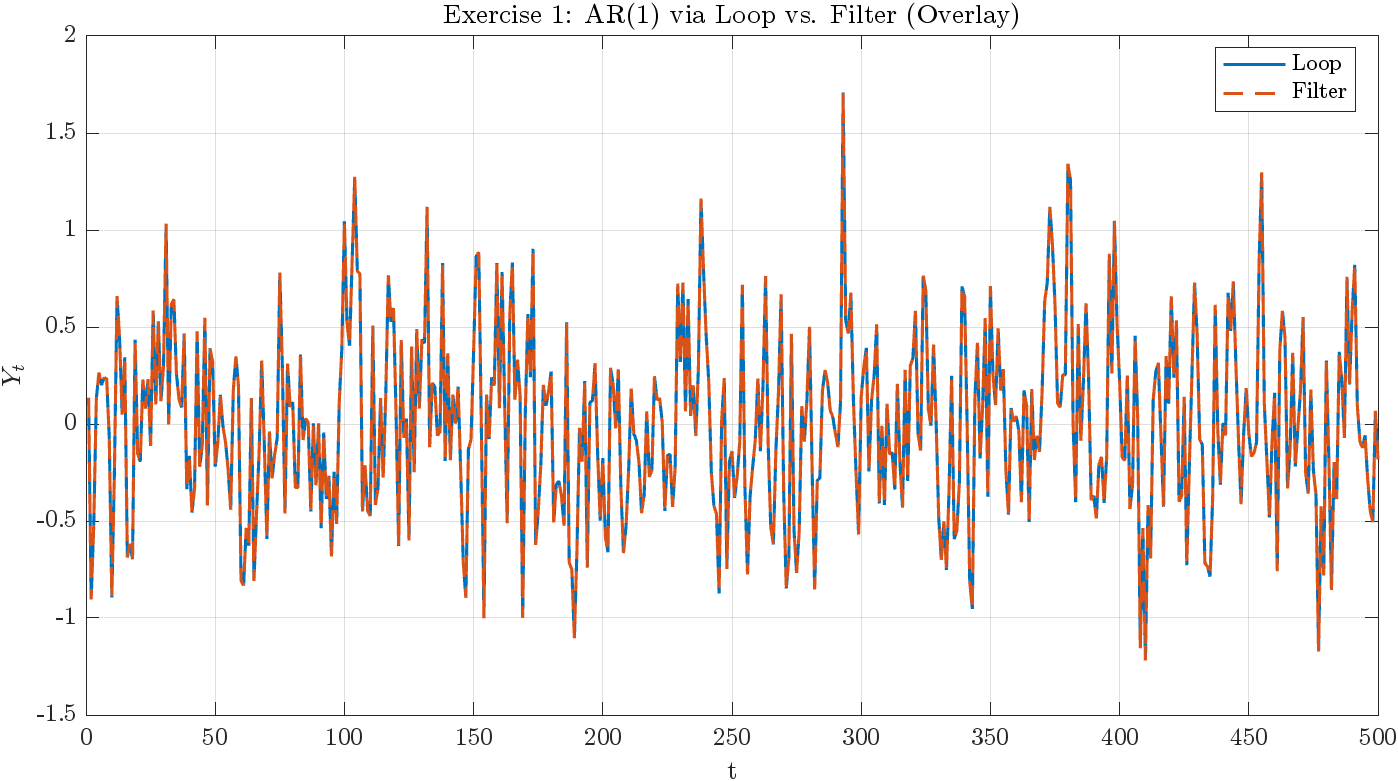
\includegraphics[width=\textwidth, trim=0cm 0cm 0cm 0.55cm, clip]{images/ex1_overlay.png}
                         \caption{Representation of the two series}
                         \label{fig:ex1_overlay}
                         
                     \end{subfigure}
                     \hfill
                     \begin{subfigure}[b]{0.99\textwidth}
                         \centering
                         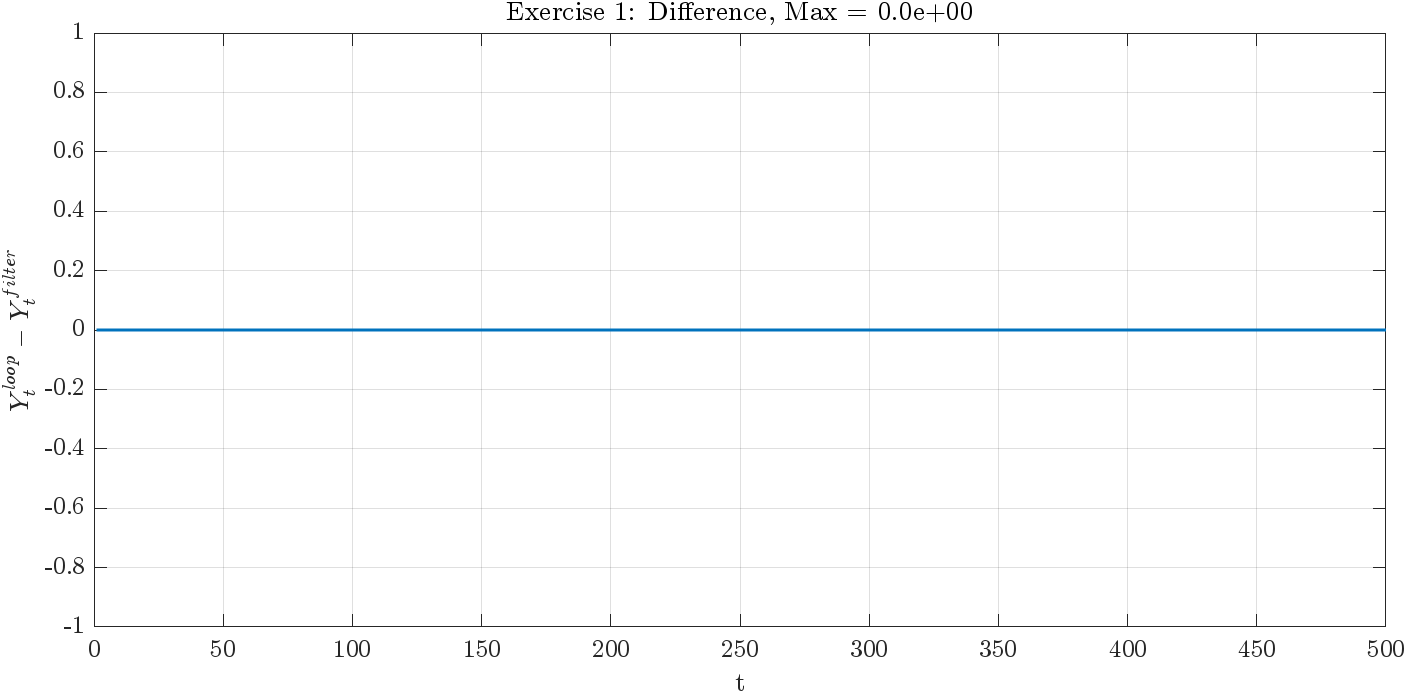
\includegraphics[width=\textwidth, trim=0cm 0cm 0cm 0.6cm, clip]{images/ex1_difference.png}
                         \caption{Representation of the \(\Delta\)}
                         \label{fig:ex1_difference}
                     \end{subfigure}
                        \label{fig:ex_1c}
                        \caption{Visual representations supporting the statement that the two series are equivalent}
                \end{figure}
        
            \end{solution}  

    \end{enumerate}

\section*{Question 2}
\setcounter{section}{2}

    Generate data from an AR(1) with $\phi=0.6$, $\sigma_\varepsilon^2=0.4$ and $\mathbb{E}[Y_t]=3$. Set the starting condition of your simulation to $20$. What happens if the starting condition you choose is far from the unconditional mean of the process? What would you do in order to make sure that the sample path is a ``proper'' realization of the stationary process you want to simulate from? You can use either \texttt{for} or \texttt{filter}.

    \begin{solution}

        We consider the AR(1)
        \begin{equation}
            Y_t \;=\; \mu \;+\; \phi\,(Y_{t-1}-\mu) \;+\; \varepsilon_t,
            \qquad \varepsilon_t \sim \mathcal{N}(0,\sigma^2),\quad |\phi|<1,
        \end{equation}
        with parameters $\phi=0.6$, $\sigma^2=0.4$, $\mu=3$. The horizon is $T=500$ and the initial condition is set far from the mean, $Y_0=20$. A fixed random seed ensures reproducibility. \\

        Writing $X_t := Y_t-\mu$ yields $X_t=\phi X_{t-1}+\varepsilon_t$, so the exact solution is
        \begin{equation}
            X_t \;=\; \phi^t X_0 \;+\; \sum_{j=0}^{t-1} \phi^{\,j}\,\varepsilon_{t-j},
            \qquad\text{hence}\qquad
            \mathbb{E}[Y_t \mid Y_0] \;=\; \mu \;+\; \phi^t\,(Y_0-\mu).
        \end{equation}
        With $\phi=0.6$ and $Y_0-\mu=17$, the deterministic component $\phi^t(Y_0-\mu)$ decays geometrically: the half-life is
        $h=\log(1/2)/\log(\phi)\approx 1.36$ periods, so the expected path returns rapidly toward $\mu=3$.
        Figure \ref{fig:ex2_path_far_from_mean} shows a simulated trajectory together with the unconditional mean.

\begin{lstlisting}[language=Matlab]
% AR(1) with phi=0.6, sigma^2=0.4, E[Y_t]=3, start Y0=20

rng(23456,'twister');              % Reproducibility for Ex.2
T      = 500;
phi2   = 0.6;
sigma2_2 = 0.4;
mu2    = 3;        % unconditional mean
Y0_far = 20;       % starting far from mean

% Simulate with a for-loop (explicit control over initial condition)
eps2 = sqrt(sigma2_2) * randn(T,1);
Y2   = simulate_ar1_loop(T, phi2, sigma2_2, mu2, Y0_far, eps2);

% Plot the sample path and the unconditional mean
fh3 = figure('Position',[100 100 900 360]);
plot(1:T, Y2, '-', 'DisplayName','$Y_t$'); hold on; grid on
yline(mu2, '--', '$\mathrm{E}[Y_t]=\mu=3$', 'Interpreter','latex', 'LabelVerticalAlignment','bottom', 'DisplayName', '$\mathrm{E}[Y_t]=\mu=3$')
xlabel('t'); ylabel('$Y_t$')
title('Exercise 2: AR(1) Path with Initial Condition Far from Mean')
legend('Location','best')
exportFig(fh3,'ex2_path_far_from_mean.png');
\end{lstlisting}

                To obtain a draw that is effectively free of initial-condition transients, we simulate $T+B$ periods and discard the first $B$ (burn-in). Since $|\phi|<1$, the effect of $Y_0$ on $Y_t$ is proportional to $\phi^t$; choosing $B=500$ makes $\phi^B$ negligible. The retained segment $\{Y_{B+1},\dots,Y_{B+T}\}$ is therefore well-approximated by a sample from the stationary distribution. Figure \ref{fig:ex2_path_after_burnin} displays the post--burn-in path with the mean line.

\begin{lstlisting} [language=Matlab]
% "Proper" stationary realization: use burn-in and then drop it
B   = 500;                              % burn-in length
TT  = T + B;
eps2b = sqrt(sigma2_2) * randn(TT,1);
Y2b    = simulate_ar1_loop(TT, phi2, sigma2_2, mu2, Y0_far, eps2b);
Y2_stat = Y2b(B+1:end);                 % drop initial transient

% Plot the post-burn-in sample path and the mean
fh4 = figure('Position',[100 100 900 360]);
plot(1:T, Y2_stat, '-', 'DisplayName','$Y_t$ after burn-in'); hold on; grid on
yline(mu2, '--', '$\mathrm{E}[Y_t]=\mu=3$', 'Interpreter','latex', 'LabelVerticalAlignment','bottom', 'DisplayName', '$\mathrm{E}[Y_t]=\mu=3$')
xlabel('t'); ylabel('$Y_t$')
title(sprintf('Exercise 2: Stationary Sample Path After Burn-in (B = %d)',B))
legend('Location','best')
exportFig(fh4,'ex2_path_after_burnin.png');
\end{lstlisting}

                \begin{figure}[h]
                     \centering
                     \begin{subfigure}[b]{0.49\textwidth}
                         \centering
                         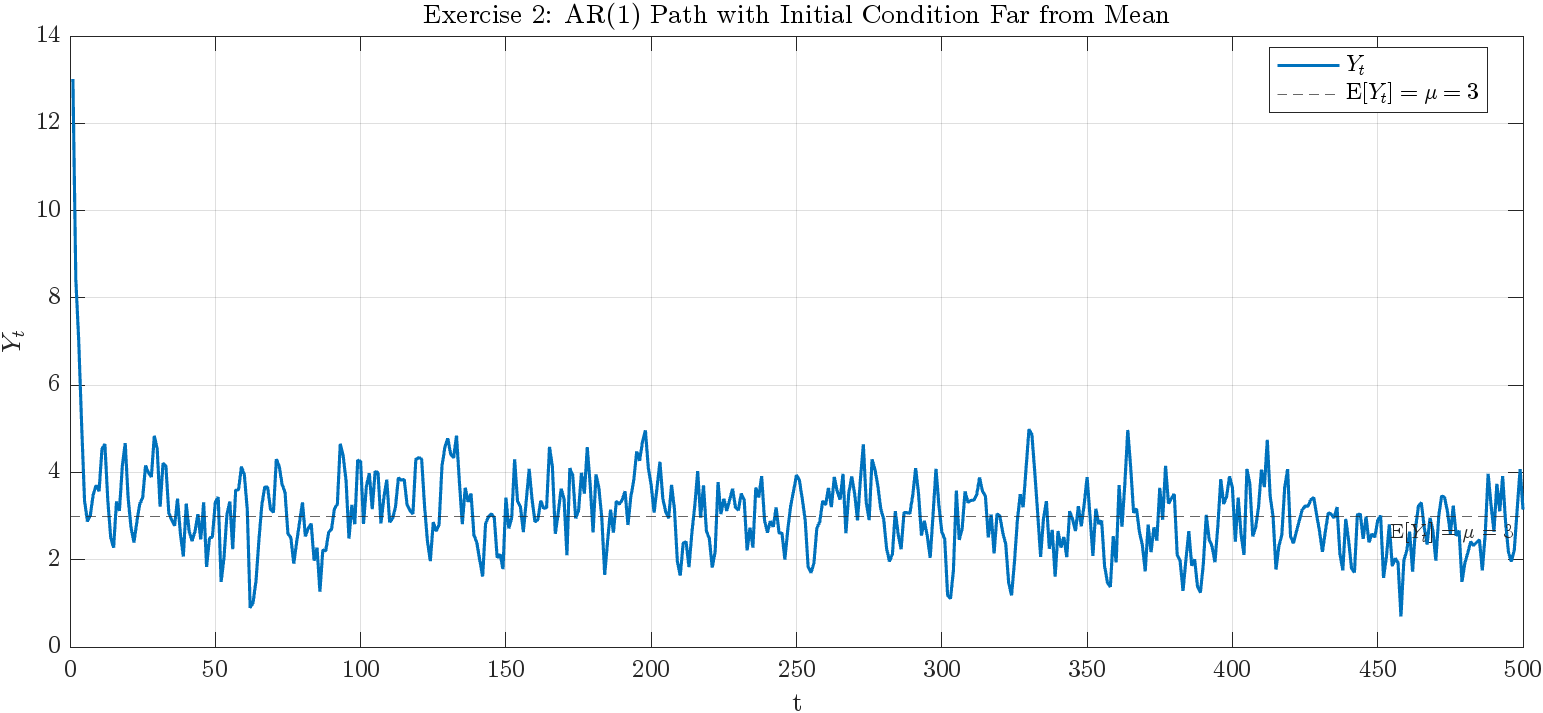
\includegraphics[width=\textwidth, trim=0cm 0cm 0cm 0.55cm, clip]{images/ex2_path_far_from_mean.png}
                         \caption{Representation of the two series}
                         \label{fig:ex2_path_far_from_mean}                         
                     \end{subfigure}
                     \hfill
                     \begin{subfigure}[b]{0.49\textwidth}
                         \centering
                         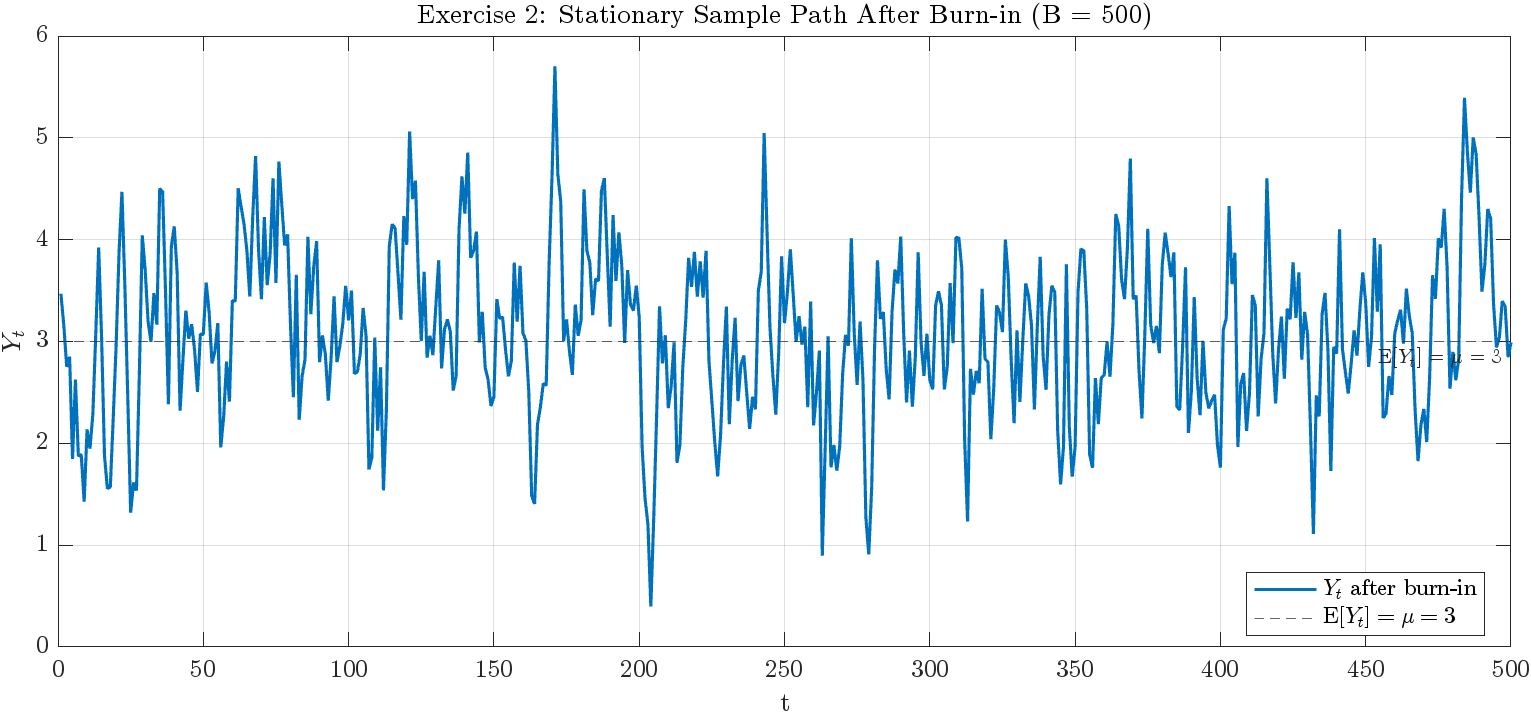
\includegraphics[width=\textwidth, trim=0cm 0cm 0cm 0.55cm, clip]{images/ex2_path_after_burnin.png}
                         \caption{Representation of the \(\Delta\)}
                         \label{fig:ex2_path_after_burnin}
                     \end{subfigure}
                        \label{fig:ex_1c}
                        \caption{Visual representations supporting the statement that the two series are equivalent}
                \end{figure}
        
    \end{solution}

\section*{Question 3}
\setcounter{section}{3}

    Compute the empirical distribution of the OLS estimator in the case of an AR(1) with $\phi=0.4$ and $T=250$ (you are free to choose the variance of the innovation). Construct a $t$-test for the null hypothesis $H_0:\ \phi=0$, against a two-sided alternative $H_1:\ \phi\neq 0$. How often do you reject $H_0$ at the 95\% confidence level when $T=250$?

    \begin{solution}

        We consider the AR(1) data-generating process (DGP)
        \begin{equation}
            Y_t \;=\; \phi\,Y_{t-1} \;+\; \varepsilon_t, \qquad \varepsilon_t \sim \mathcal{N}(0,\sigma^2), 
        \end{equation}
        with $\phi=0.4$, $\sigma^2=1$, and $T=250$. To remove transients from the initial condition, each replication simulates $T+B$ observations with a burn-in of $B=300$ and retains the last $T$ points.\footnote{With $|\phi|<1$, the effect of $Y_0$ on $Y_t$ decays like $\phi^t$; a burn-in of 300 makes this negligible.} We run $R=5000$ replications.

\begin{lstlisting}[language=Matlab]
% Empirical distribution of OLS estimator; t-test of H0: phi=0
% DGP: AR(1) with phi=0.4, T=250.

rng(34567,'twister');
T      = 250;
phi3   = 0.4;
sigma2_3 = 1.0;      % explicit
mu3    = 0;
R      = 5000;       % number of Monte Carlo replications
B      = 300;        % short burn-in for stationarity

phi_hat = zeros(R,1);
tstat   = zeros(R,1);
\end{lstlisting}

        In each replication we estimate $\phi$ by OLS from the regression $Y_t=\phi Y_{t-1}+u_t$ (no constant since the DGP has mean zero):
        \[
          \widehat\phi \;=\; 
          \frac{\sum_{t=2}^T Y_{t-1}Y_t}{\sum_{t=2}^T Y_{t-1}^2},
          \qquad 
          \widehat u_t \;=\; Y_t-\widehat\phi\,Y_{t-1}.
        \]
        Let $\widehat s^2=\sum_{t=2}^T \widehat u_t^2/(T-1)$ and
        $\operatorname{se}(\widehat\phi)=\sqrt{\widehat s^2/\sum_{t=2}^T Y_{t-1}^2}$.
        We test $H_0\!:\phi=0$ with the usual $t$-statistic
        \[
          t \;=\; \frac{\widehat\phi-0}{\operatorname{se}(\widehat\phi)},
        \]
        and reject for $|t|>t_{0.975,T-1}$ (two-sided 5\%).

\begin{lstlisting}[language=Matlab]
for r = 1:R
    % Innovations and simulation length with burn-in
    TT   = T + B;
    eps3 = sqrt(sigma2_3) * randn(TT,1);

    % Start at the mean (mu3) + burn-in
    Ytmp = simulate_ar1_loop(TT, phi3, sigma2_3, mu3, mu3, eps3);
    Y    = Ytmp(B+1:end);                 % keep last T observations

    % OLS in Y_t = phi * Y_{t-1} + u_t  (no intercept; mean is zero)
    ylag = Y(1:end-1);
    yt   = Y(2:end);
    X    = ylag;                           % (T-1) x 1
    bhat = (X' * X) \ (X' * yt);
    uhat = yt - X * bhat;

    % --- Correct degrees of freedom: nu = (T-1) - 1 = T - 2 ---
    nu   = (T - 1) - 1;
    s2   = (uhat' * uhat) / nu;            % unbiased sigma_u^2
    se   = sqrt( s2 / (X' * X) );          % std error of bhat

    phi_hat(r) = bhat;
    tstat(r)   = bhat / se;                % test H0: phi = 0
end
\end{lstlisting}

        The Monte Carlo summary reports the empirical mean and standard deviation of $\widehat\phi$ across replications and the rejection frequency at the 5\% level. In our run, the mean of $\widehat\phi$ is slightly below the true value (a familiar small finite-sample downward bias for positive $\phi$), while the 5\% test of $H_0\!:\phi=0$ rejects essentially always, reflecting very high power at $T=250$ and $\phi=0.4$.

        \begin{remark}
            As $T\to\infty$, $\sqrt{T}(\widehat\phi-\phi)\overset{d}{\to}\mathcal{N}\!\left(0,\,1-\phi^2\right)$, so, under $H_1\!:\phi\neq0$, the $t$-statistic is approximately normal with noncentrality
            \[
              \lambda \;\approx\; \frac{\phi}{\sqrt{(1-\phi^2)/T}}
              \;=\; \phi\,\sqrt{\frac{T}{1-\phi^2}}.
            \]
            For $\phi=0.4$ and $T=250$, this gives $\lambda\approx 6.9$, implying near–unit power, consistent with the simulated rejection rate.
        \end{remark}

\begin{lstlisting}[language=Matlab]
% Rejection frequency at 5%
if exist('tinv','file')
    tcrit = tinv(0.975, nu);
else
    tcrit = 1.96; % approximation for moderate T
end
reject = mean(abs(tstat) > tcrit);

% Report
fprintf('[Ex.3] Monte Carlo with R=%d, T=%d: mean(phi_hat)=%.4f, sd(phi_hat)=%.4f, reject H0 at 5%% = %.3f\n', ...
    R, T, mean(phi_hat), std(phi_hat), reject);

% Save a small summary table
MC_tbl = table(mean(phi_hat), std(phi_hat), reject, 'VariableNames', ...
    {'mean_phi_hat','sd_phi_hat','reject_H0_rate'});
writetable(MC_tbl, fullfile(outdir,'ex3_summary.csv')); % CSV
\end{lstlisting}

        \begin{table}[h]
            \centering
            \begin{tabular}{l c}
                \hline
                Mean $(\hat{\phi})$ & 0.3949 \\
                Standard Deviation $(\hat{\phi})$ & 0.0589 \\
                reject\_H0\_rate & 1 \\
                \hline
            \end{tabular}
            \caption{Summary statistics}
            \label{tab:phi_hat_summary}
        \end{table}

        \begin{figure}[h]
            \centering
            \caption{The histogram below depicts the empirical sampling distribution of $\widehat\phi$ across the $R$ replications, with vertical lines at the true value $\phi=0.4$ and at the Monte Carlo mean $\mathrm{mean}(\widehat\phi)$.}
            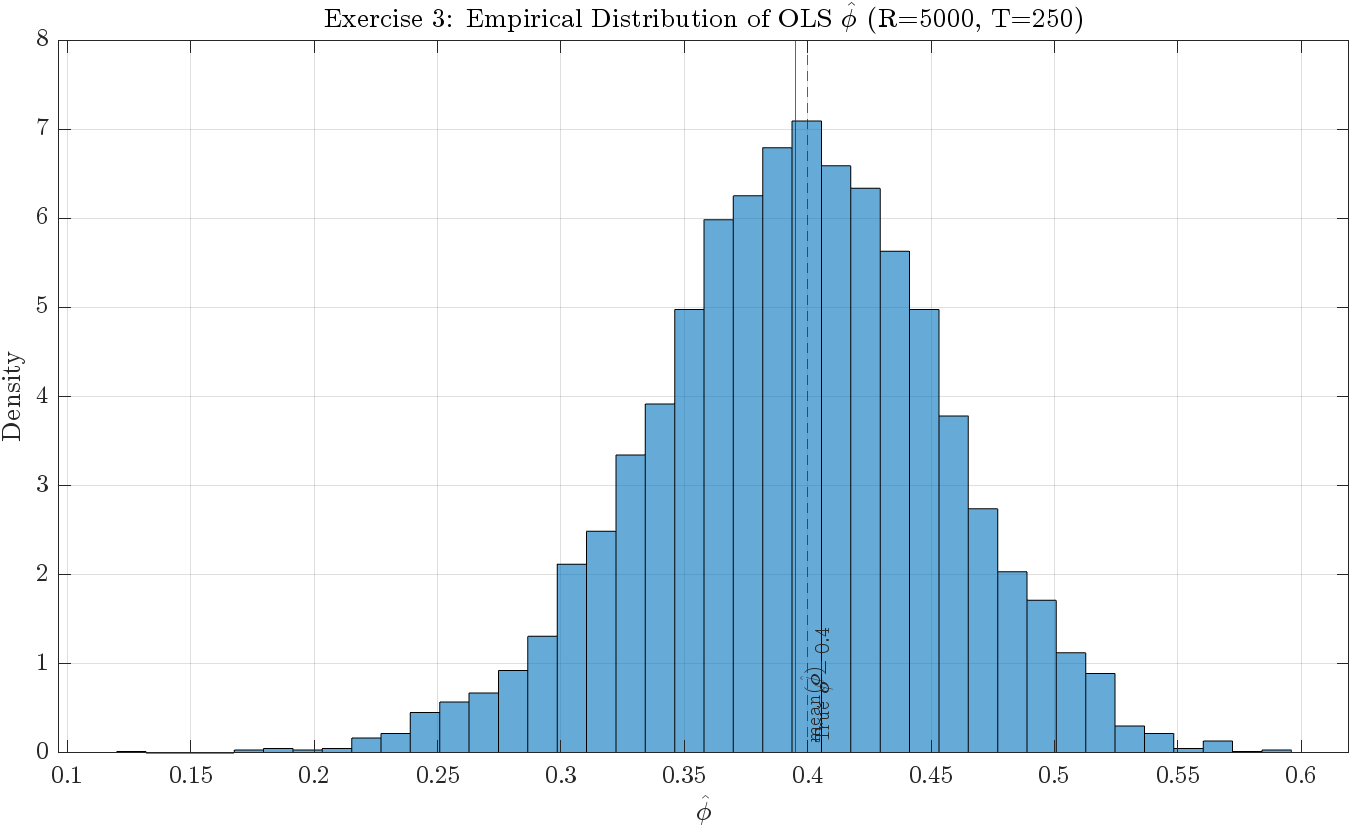
\includegraphics[width=0.99\linewidth]{images/ex3_phi_hat_hist.png}
            \label{fig:ex3_phi_hat_hist}
        \end{figure}

\begin{lstlisting}[language=Matlab]
% Histogram of phi_hat with reference lines
fh5 = figure('Position',[100 100 800 420]);
histogram(phi_hat, 40, 'Normalization','pdf'); hold on; grid on
xline(phi3, '--', 'True $\phi=0.4$', 'LabelVerticalAlignment','bottom', 'Interpreter','latex');
xline(mean(phi_hat), '-', '$\mathrm{mean}(\hat{\phi})$', 'LabelVerticalAlignment','bottom', 'Interpreter','latex');
xlabel('$\hat{\phi}$'); ylabel('Density')
title(['Exercise 3: Empirical Distribution of OLS ', '$\hat{\phi}$', ' (R=', num2str(R), ', T=', num2str(T), ')'], 'Interpreter','latex')
exportFig(fh5,'ex3_phi_hat_hist.png');
\end{lstlisting}
        
    \end{solution}

\section*{Question 4}
\setcounter{section}{4}

    Compute the empirical distribution of the OLS estimator in the case of an AR(1) with $\phi=0.9$ and $T\in\{50,100,200,1000\}$. For each $T$, do $1000$ simulations and plot the distribution. How is the distribution changing with $T$?

    \begin{solution}

        For each sample size $T\in\{50,100,200,1000\}$ we simulate $R=1000$ samples, discarding a burn–in of $B=500$ observations to remove dependence on initial conditions. For each replication we compute the OLS estimator from the regression through the origin (consistent with $\mu=0$):
        \[
        \widehat\phi=\frac{\sum_{t=2}^{T} y_{t-1}y_t}{\sum_{t=2}^{T} y_{t-1}^2}.
        \]
        We also record the usual OLS standard error and $t$-statistic for testing $H_0:\phi=0$ (formally using $n=T-1$ observations and $\nu=n-1=T-2$ degrees of freedom). \\

        In our notes, the least-squares probability limit for an AR(1) is
        \[
        \operatorname*{plim}\ \widehat\phi \;=\; \frac{\gamma_1}{\gamma_0}\;=\;\phi,
        \]
        where $\gamma_h=\operatorname{Cov}(y_t,y_{t-h})$. Thus $\widehat\phi$ is consistent. Moreover, under standard regularity conditions,
        \[
        \sqrt{T}\,(\widehat\phi-\phi)\ \xrightarrow{d}\ \mathcal{N}\!\left(0,\ 1-\phi^2\right),
        \]
        so that, asymptotically,
        \[
        \operatorname{sd}(\widehat\phi)\ \approx\ \sqrt{\frac{1-\phi^2}{T}}.
        \]
        For $\phi=0.9$, $1-\phi^2=0.19$, so $\operatorname{sd}(\widehat\phi)\approx \sqrt{0.19/T}$. \\

        The Monte Carlo follows exactly this design:
        
        \begin{enumerate}
            \item Draw $\{\varepsilon_t\}_{t=1}^{T+B}$ i.i.d.\ $\mathcal{N}(0,1)$.
          
            \item Generate $\{y_t\}$ recursively with the given $\phi$, keep the last $T$ observations after the burn–in.
          
            \item Compute $\widehat\phi$ via the no-intercept OLS formula above.
          
            \item For inference quantities, use $n=T-1$ effective observations and an unbiased residual variance estimator $\widehat\sigma^2=\text{RSS}/(n-1)=\text{RSS}/(T-2)$, which implies $\operatorname{se}(\widehat\phi)=\sqrt{\widehat\sigma^2/\sum y_{t-1}^2}$ and $t$-critical values based on $\nu=T-2$ degrees of freedom.
        \end{enumerate}

\begin{lstlisting}[language=Matlab]
% Empirical distribution of OLS AR(1) with phi = 0.9 over varying T

rng(45678,'twister');                % Reproducibility for Ex.4
phi      = 0.9;
sigma2_4 = 1.0;                      % Var(eps_t)
mu       = 0;
Ts       = [50, 100, 200, 1000];
R        = 1000;
B        = 500;                      % burn-in to reduce dependence on start

E4_summary = table('Size',[numel(Ts) 5], ...
    'VariableTypes',{'double','double','double','double','double'}, ...
    'VariableNames',{'T','mean_phi_hat','sd_phi_hat','bias','rej_H0_phi0_rate'});

for iT = 1:numel(Ts)
    T = Ts(iT);
    nu = T - 2;                      % df for regression with (T-1) rows, 1 slope

    phi_hat = zeros(R,1);
    tstat   = zeros(R,1);

    for r = 1:R
        % --- simulate AR(1) with burn-in
        TT   = T + B;
        eps  = sqrt(sigma2_4) * randn(TT,1);
        Yall = simulate_ar1_loop(TT, phi, sigma2_4, mu, mu, eps);
        Y    = Yall(B+1:end);        % keep last T observations

        % --- OLS: Y_t = phi * Y_{t-1} + u_t (no intercept since mu=0)
        ylag = Y(1:end-1); 
        yt   = Y(2:end);
        X    = ylag;                  % (T-1)-by-1 regressor
        XX   = X' * X;

        bhat = XX \ (X' * yt);
        uhat = yt - X * bhat;

        % --- correct finite-sample variance and t-stat
        s2 = (uhat' * uhat) / nu;     % unbiased residual variance: RSS/(T-2)
        se = sqrt( s2 / XX );         % std error of slope
        tstat(r)   = bhat / se;       % test H0: phi = 0
        phi_hat(r) = bhat;
    end

    % --- Monte Carlo summaries for this T
    m    = mean(phi_hat);
    sd   = std(phi_hat);
    bias = m - phi;

    if exist('tinv','file')
        tcrit = tinv(0.975, nu);      % two-sided 5% test against H0: phi = 0
    else
        tcrit = 1.96;                 % normal approx
    end
    rej = mean(abs(tstat) > tcrit);

    E4_summary{iT,:} = [T, m, sd, bias, rej];

    % --- Histogram for this T
    fh = figure('Position',[100 100 840 420]);
    histogram(phi_hat, 40, 'Normalization','pdf'); hold on; grid on
    xline(phi, '--', 'True $\phi=0.9$', 'LabelVerticalAlignment','bottom', 'Interpreter','latex');
    xline(m,  '-',  '$\mathrm{mean}(\hat{\phi})$', 'LabelVerticalAlignment','bottom', 'Interpreter','latex');
    xlabel('$\hat{\phi}$', 'Interpreter','latex'); 
    ylabel('Density', 'Interpreter','latex');
    title(sprintf('Exercise 4: OLS on AR(1), $\\phi=0.9$ (T=%d, R=%d)', T, R), 'Interpreter','latex');
    exportFig(fh, sprintf('ex4_hist_T%d.png', T));
end

% Save table
writetable(E4_summary, fullfile(outdir,'ex4_summary.csv'));
\end{lstlisting}

        From the $R=1000$ replications we obtain, for each $T$, the Monte Carlo mean, standard deviation, and bias (mean minus $0.9$). The reported summary is:
        
        \begin{center}
            \begin{tabular}{rcccc}
                \toprule
                $T$ & $\mathrm{mean}(\widehat\phi)$ & $\mathrm{sd}(\widehat\phi)$ & $\mathrm{bias}$ & $\mathrm{rej}\{H_0\!:\phi=0\}$ \\
                \midrule
                $50$   & $0.8682$ & $0.0756$ & $-0.0318$ & $1.000$\\
                $100$  & $0.8840$ & $0.0493$ & $-0.0160$ & $1.000$\\
                $200$  & $0.8908$ & $0.0322$ & $-0.0092$ & $1.000$\\
                $1000$ & $0.8983$ & $0.0138$ & $-0.0017$ & $1.000$\\
                \bottomrule
            \end{tabular}
        \end{center}
        
        Two key comparisons with the asymptotic variance formula help interpret these numbers. Theoretical $\operatorname{sd}(\widehat\phi)\approx\sqrt{0.19/T}$ yields $0.062$ ($T{=}50$), $0.044$ ($T{=}100$), $0.031$ ($T{=}200$), and $0.0138$ ($T{=}1000$). The Monte Carlo standard deviations are close and converge toward these values as $T$ grows (the mild over-dispersion at small $T$ is a known finite-sample feature). The Monte Carlo mean shows the familiar \emph{downward} small-sample bias for $\phi>0$, which is $O(1/T)$ and vanishes as $T$ increases.

                \begin{figure}[h]
                     \centering
                     \begin{subfigure}[b]{0.49\textwidth}
                         \centering
                         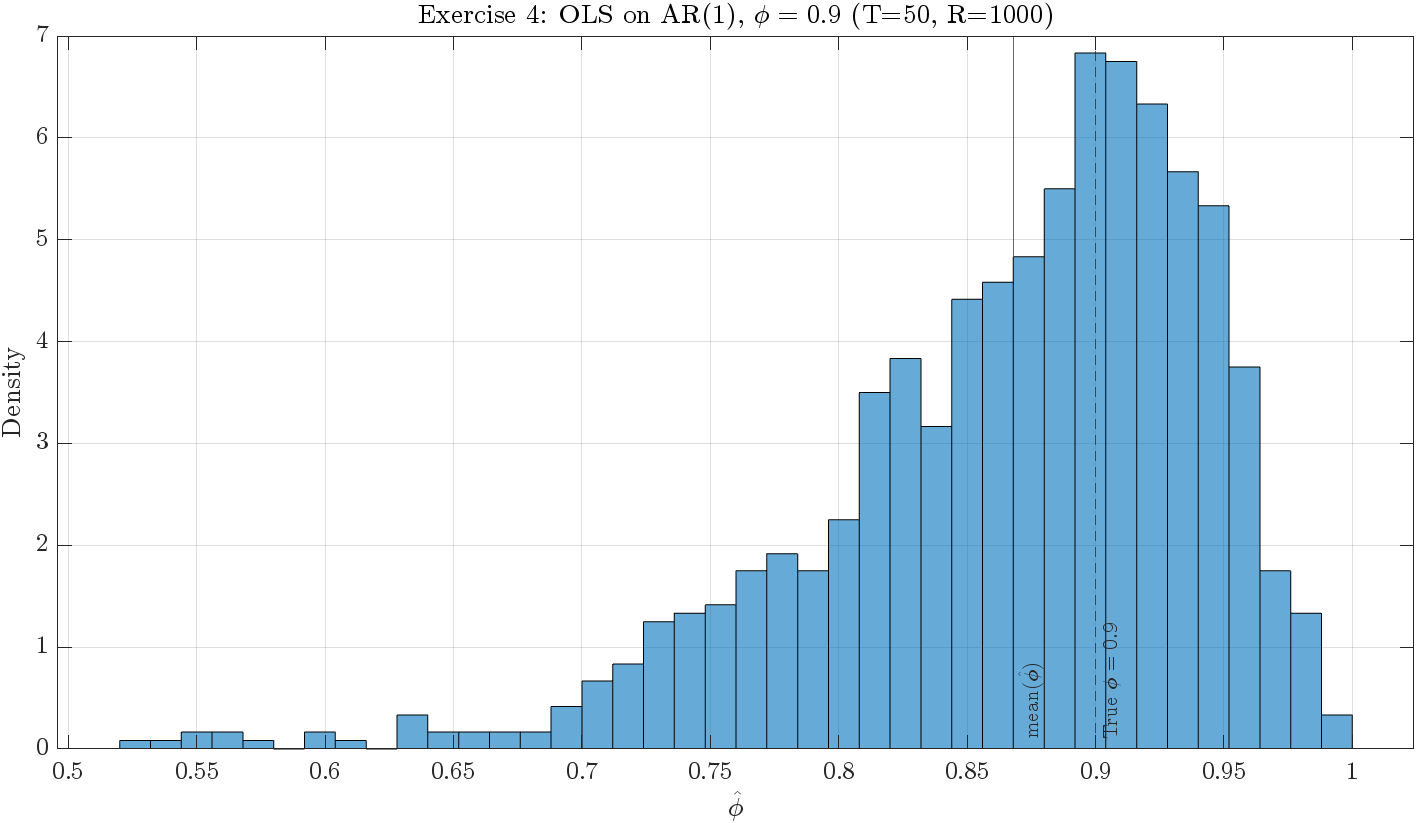
\includegraphics[width=\textwidth, trim=0cm 0cm 0cm 0.55cm, clip]{images/ex4_hist_T50.png}
                         \caption{\(T=50\)}
                         \label{fig:ex4_hist_T50}                         
                     \end{subfigure}
                     \hfill
                     \begin{subfigure}[b]{0.49\textwidth}
                         \centering
                         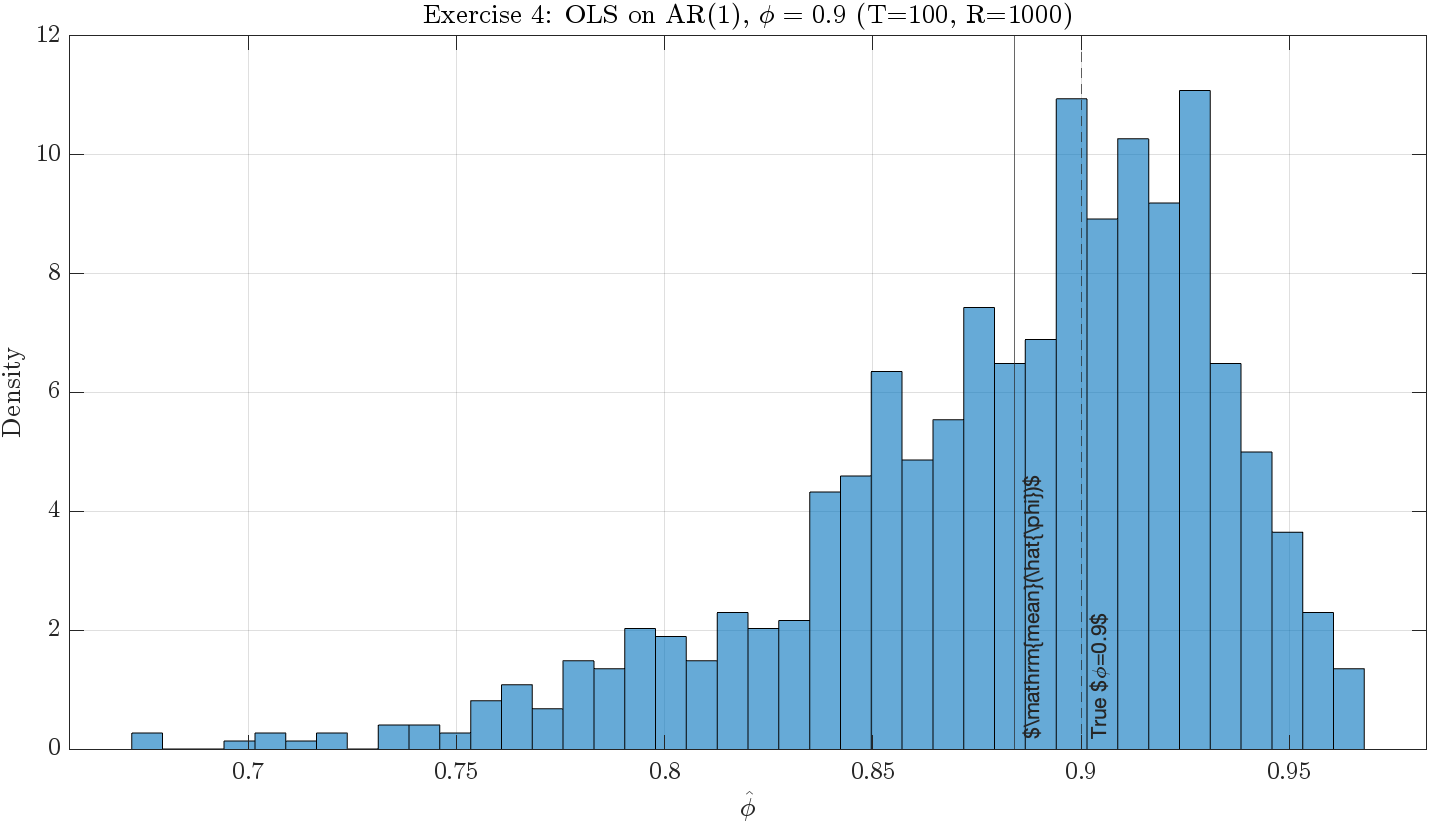
\includegraphics[width=\textwidth, trim=0cm 0cm 0cm 0.55cm, clip]{images/ex4_hist_T100.png}
                         \caption{\(T=100\)}
                         \label{fig:ex2_path_after_burnin}
                     \end{subfigure}
                     \hfill
                     \begin{subfigure}[b]{0.49\textwidth}
                         \centering
                         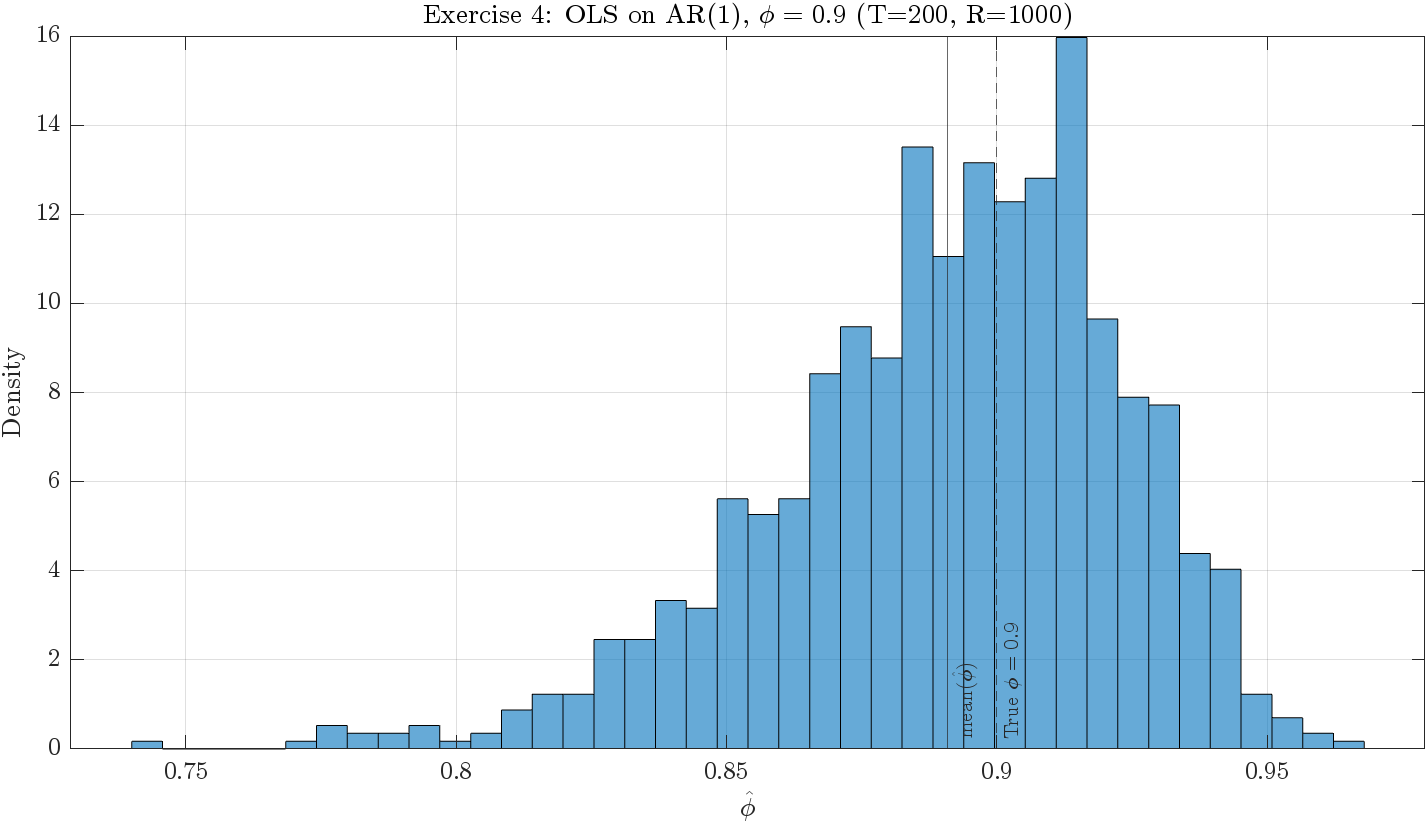
\includegraphics[width=\textwidth, trim=0cm 0cm 0cm 0.55cm, clip]{images/ex4_hist_T200.png}
                         \caption{\(T=200\)}
                         \label{fig:ex2_path_after_burnin}
                     \end{subfigure}
                     \hfill
                     \begin{subfigure}[b]{0.49\textwidth}
                         \centering
                         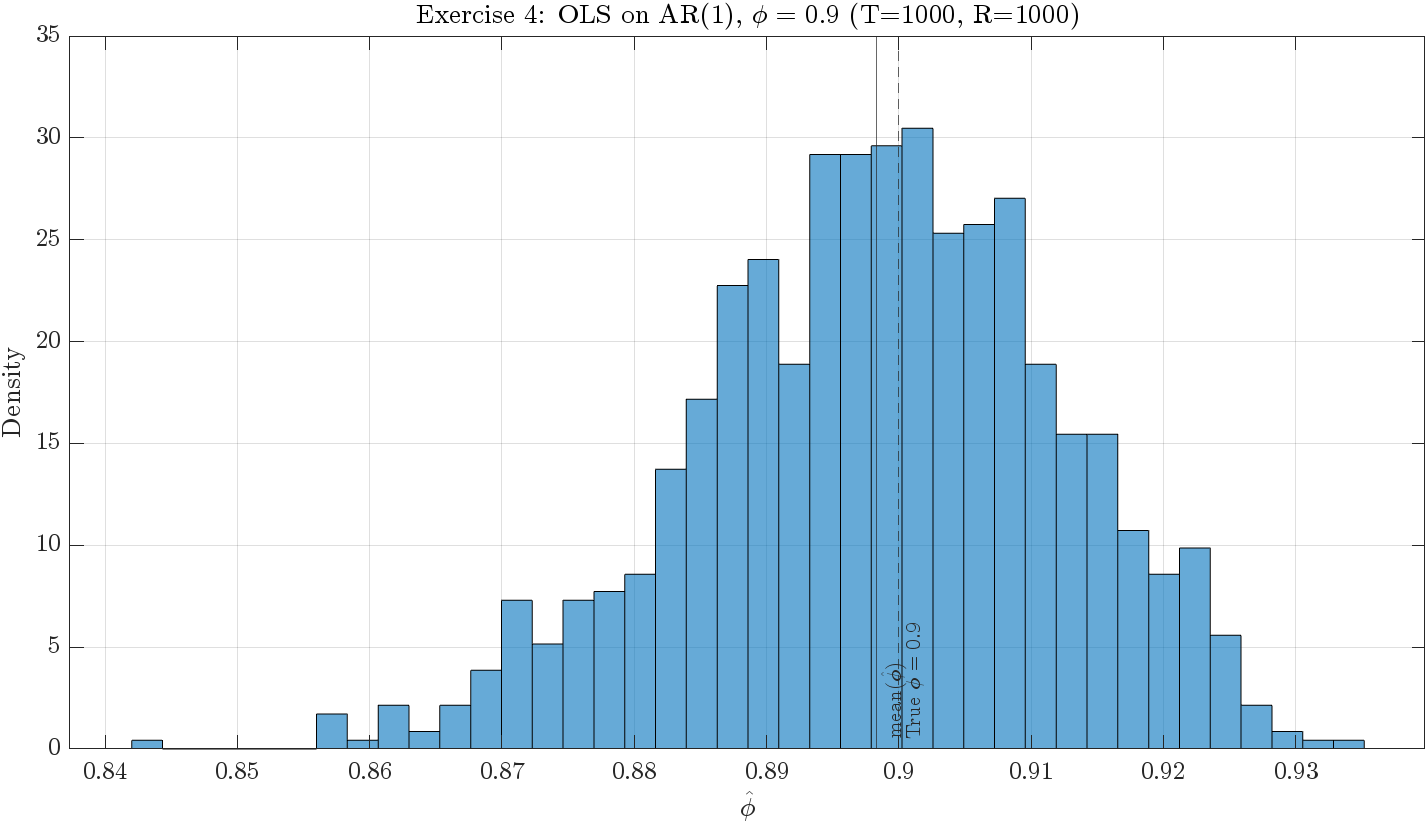
\includegraphics[width=\textwidth, trim=0cm 0cm 0cm 0.55cm, clip]{images/ex4_hist_T1000.png}
                         \caption{\(T=1000\)}
                         \label{fig:ex2_path_after_burnin}
                     \end{subfigure}
                    \label{fig:ex_1c}
                    \caption{Evolution of the distributions as the number of observations \(T\) increases.}
                \end{figure}

        The histograms (one per $T$) and the table convey the same message:
        
        \begin{itemize}
            \item \textbf{Centering:} The distribution is centered below $\phi$ for small $T$ (negative finite-sample bias), but the bias shrinks rapidly (from about $-0.032$ at $T=50$ to about $-0.002$ at $T=1000$), in line with consistency.
          
            \item \textbf{Spread:} The dispersion decreases roughly at the $\propto T^{-1/2}$ rate. Numerically, the standard deviation falls from $\approx0.076$ ($T=50$) to $\approx0.014$ ($T=1000$), very close to $\sqrt{(1-\phi^2)/T}$.
          
            \item \textbf{Shape:} By the central limit reasoning above, the standardized estimator $\sqrt{T}(\widehat\phi-\phi)$ becomes approximately normal as $T$ increases. Empirically, the histograms become more symmetric and concentrated around $0.9$ as $T$ grows, with thinner tails.
        \end{itemize}
        
    \end{solution}

\section*{Question 5}
\setcounter{section}{5}

    Compute the empirical distribution (do $1000$ simulations) of the OLS estimator in the regression $x_t = a x_{t-1} + v_t$ in the case in which the data-generating process for $x_t$ is MA(1) with $\theta=0.6$ for $T\in\{50,100,200,1000\}$. What is the mean of the distributions? Does the mean converge to anything as $T\to\infty$? Discuss.

    \begin{solution}

        We simulate MA(1) data
        \[
        x_t \;=\; \varepsilon_t + \theta \varepsilon_{t-1},\qquad \varepsilon_t\stackrel{i.i.d.}{\sim}\mathcal{N}(0,\sigma^2),\ \theta=0.6,
        \]
        keep the last $T$ observations after a burn-in of $B=500$, and estimate, for each replication,
        \[
        \hat a \;=\; \arg\min_a \sum_{t=2}^{T}\big(x_t-a\,x_{t-1}\big)^2
        \;=\;
        \frac{\sum_{t=2}^{T} x_{t-1}x_t}{\sum_{t=2}^{T} x_{t-1}^2}.
        \]
        We repeat this $R=1000$ times for each $T$, plot the histogram of $\hat a$, and compute the Monte Carlo mean and standard deviation. \\

        Because the regression omits the MA structure, OLS converges to the \emph{projection} coefficient of $x_t$ on $x_{t-1}$:
        \[
        \operatorname{plim}\hat a
        \;=\;
        \frac{\operatorname{Cov}(x_t,x_{t-1})}{\operatorname{Var}(x_{t-1})}
        \;=\;\frac{\gamma_1}{\gamma_0}
        \;=\;\rho(1).
        \]
        For an MA(1),
        $\gamma_0=(1+\theta^2)\sigma^2$ and $\gamma_1=\theta\sigma^2$,
        so
        \[
        \operatorname{plim}\hat a \;=\; \frac{\theta}{1+\theta^2}.
        \]
        With $\theta=0.6$, this gives
        \[
        \frac{0.6}{1+0.6^2} \;=\; \frac{0.6}{1.36} \;=\; 0.441176\overline{47}.
        \]


\begin{lstlisting}[language=Matlab]
% OLS of x_t on x_{t-1} when x_t is MA(1) with theta=0.6
% DGP: x_t = eps_t + theta * eps_{t-1},  eps_t ~ N(0, sigma^2)

rng(56789,'twister');              % Reproducibility for Ex.5
theta = 0.6;
sigma2_5 = 1.0;        % explicit
Ts   = [50, 100, 200, 1000];
R    = 1000;
B    = 500;            % burn-in for MA(1)

% Theoretical plim of OLS when regressing x_t on x_{t-1}: rho(1) = theta/(1+theta^2)
plim_a = theta / (1 + theta^2);

E5_summary = table('Size',[numel(Ts) 5], ...
    'VariableTypes',{'double','double','double','double','double'}, ...
    'VariableNames',{'T','mean_a_hat','sd_a_hat','bias_from_plim','theoretical_plim'});

for iT = 1:numel(Ts)
    T = Ts(iT);
    a_hat = zeros(R,1);

    for r = 1:R
        TT   = T + B;
        % Simulate MA(1) with burn-in
        [x_all, ~] = simulate_ma1(TT, theta, sigma2_5, 0);
        x = x_all(B+1:end);

        Xlag = x(1:end-1); xt = x(2:end);
        bhat = (Xlag' * Xlag) \ (Xlag' * xt);  % no constant
        a_hat(r) = bhat;
    end

    m  = mean(a_hat);
    sd = std(a_hat);
    bias = m - plim_a;
    E5_summary{iT,:} = [T, m, sd, bias, plim_a];

    % Plot histogram for this T
    fh = figure('Position',[100 100 840 420]);
    histogram(a_hat, 40, 'Normalization','pdf'); hold on; grid on
    xline(plim_a, '--', sprintf('plim = %.3f', plim_a), 'LabelVerticalAlignment','bottom');
    xline(m,      '-',  '$\mathrm{mean}(\hat{a})$', 'LabelVerticalAlignment','bottom');
    xlabel('$\hat{a}$'); ylabel('Density')
    title(['Exercise 5: OLS on MA(1) Data, ', '$\theta=0.6$', ' (T=', num2str(T), ', R=', num2str(R), ')'], 'Interpreter','latex')
    exportFig(fh, sprintf('ex5_hist_T%d.png', T));
end

% Save table
writetable(E5_summary, fullfile(outdir,'ex5_summary.csv'));

%% From the "Helper functions" section:

function [x, eps] = simulate_ma1(T, theta, sigma2, mu)
%SIMULATE_MA1 Simulate MA(1): x_t = mu + eps_t + theta*eps_{t-1}
    if nargin < 4, mu = 0; end
    eps = sqrt(sigma2) * randn(T,1);
    % Vectorized MA(1): set eps_0 = 0 and use lagged innovations
    eps_lag = [0; eps(1:end-1)];
    x = mu + eps + theta * eps_lag;
end
\end{lstlisting}

        

        Across the $R=1000$ replications, the empirical results are as follows:
        
        \begin{table}[h]
            \centering
            \begin{tabular}{c|cccc}
                $T$ & mean$(\hat{a})$ & sd$(\hat{a})$ & Bias from \texttt{plin} & Theoretical \texttt{plim} \\ 
                \hline
                \hline
                50 & 0.434493054710814 & 0.106511187264365 & -0.00668341587742133 & 0.441176470588235 \\
                100 & 0.437911528963784 & 0.0742479286576639 & -0.00326494162445146 & 0.441176470588235 \\
                200 & 0.435441067223447 & 0.0535341394861661 & -0.00573540336478806 & 0.441176470588235 \\
                1000 & 0.439680841416116 & 0.0230883947393155 & -0.00149562917211887 & 0.441176470588235 \\
            \end{tabular}
            \caption{Summary statistics for different sample sizes $T$.}
            \label{tab:summary_statistics}
        \end{table}

        \begin{figure}[h]
                     \centering
                     \begin{subfigure}[b]{0.49\textwidth}
                         \centering
                         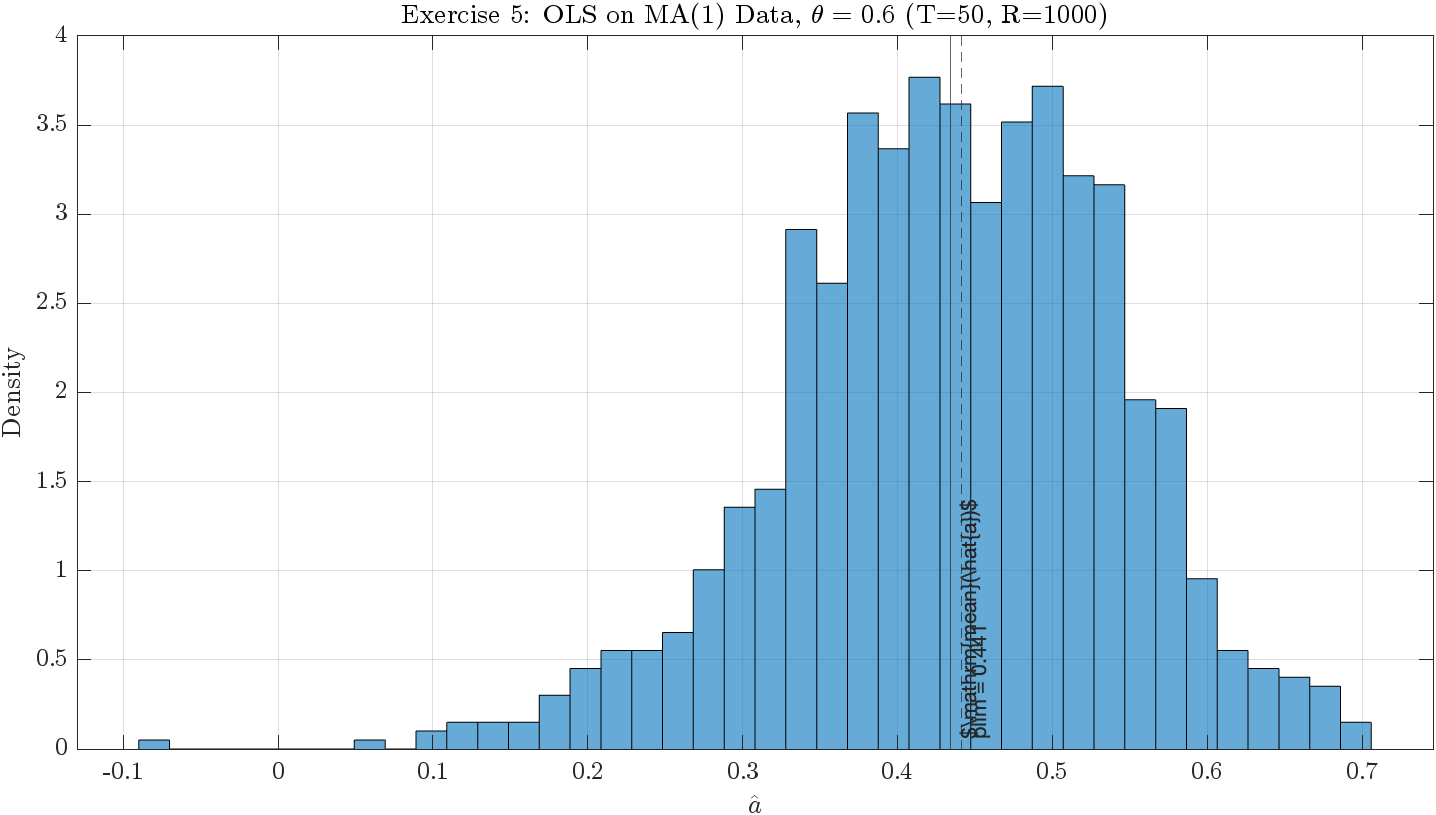
\includegraphics[width=\textwidth, trim=0cm 0cm 0cm 0.55cm, clip]{images/ex5_hist_T50.png}
                         \caption{\(T=50\)}
                         \label{fig:ex4_hist_T50}                         
                     \end{subfigure}
                     \hfill
                     \begin{subfigure}[b]{0.49\textwidth}
                         \centering
                         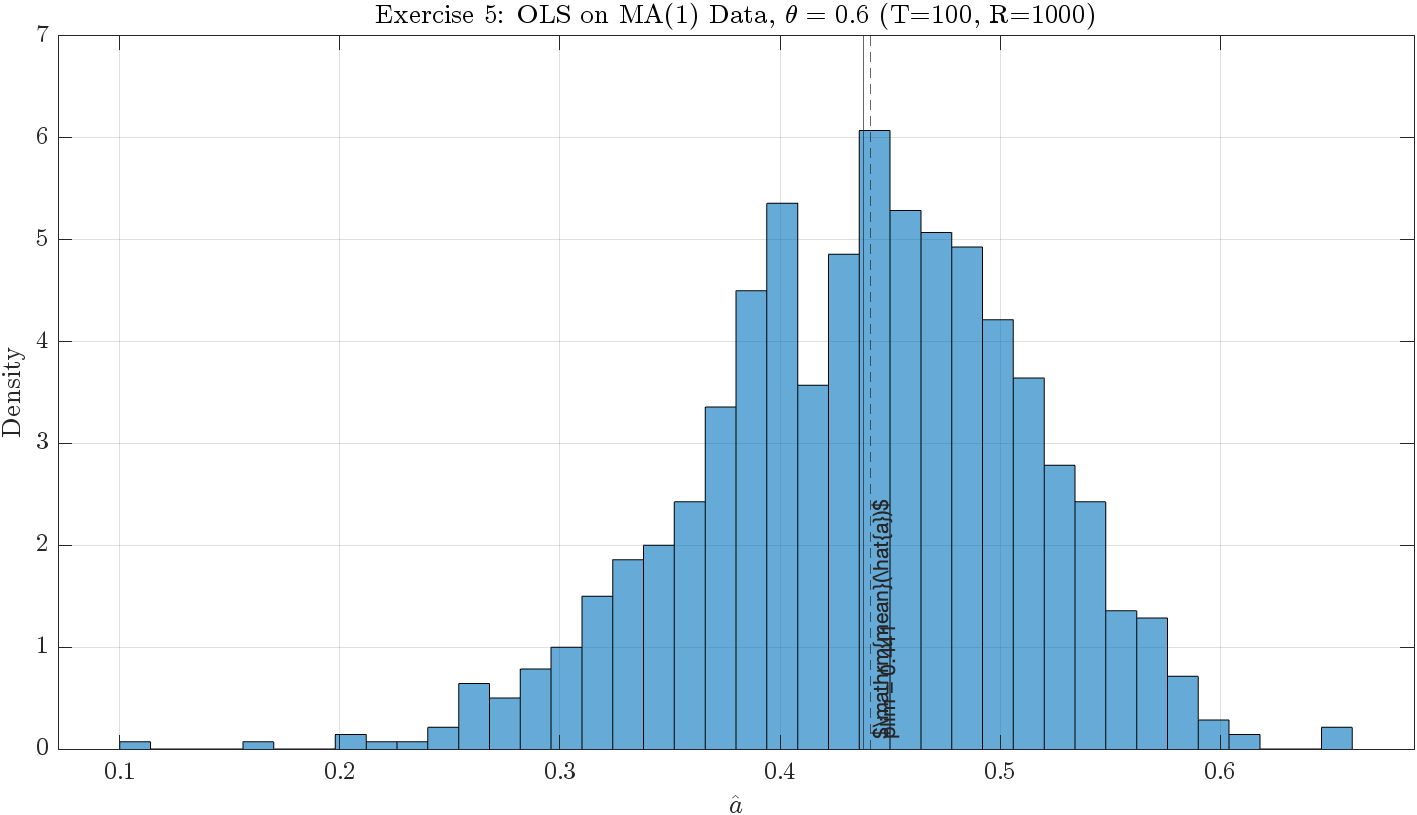
\includegraphics[width=\textwidth, trim=0cm 0cm 0cm 0.55cm, clip]{images/ex5_hist_T100.png}
                         \caption{\(T=100\)}
                         \label{fig:ex2_path_after_burnin}
                     \end{subfigure}
                     \hfill
                     \begin{subfigure}[b]{0.49\textwidth}
                         \centering
                         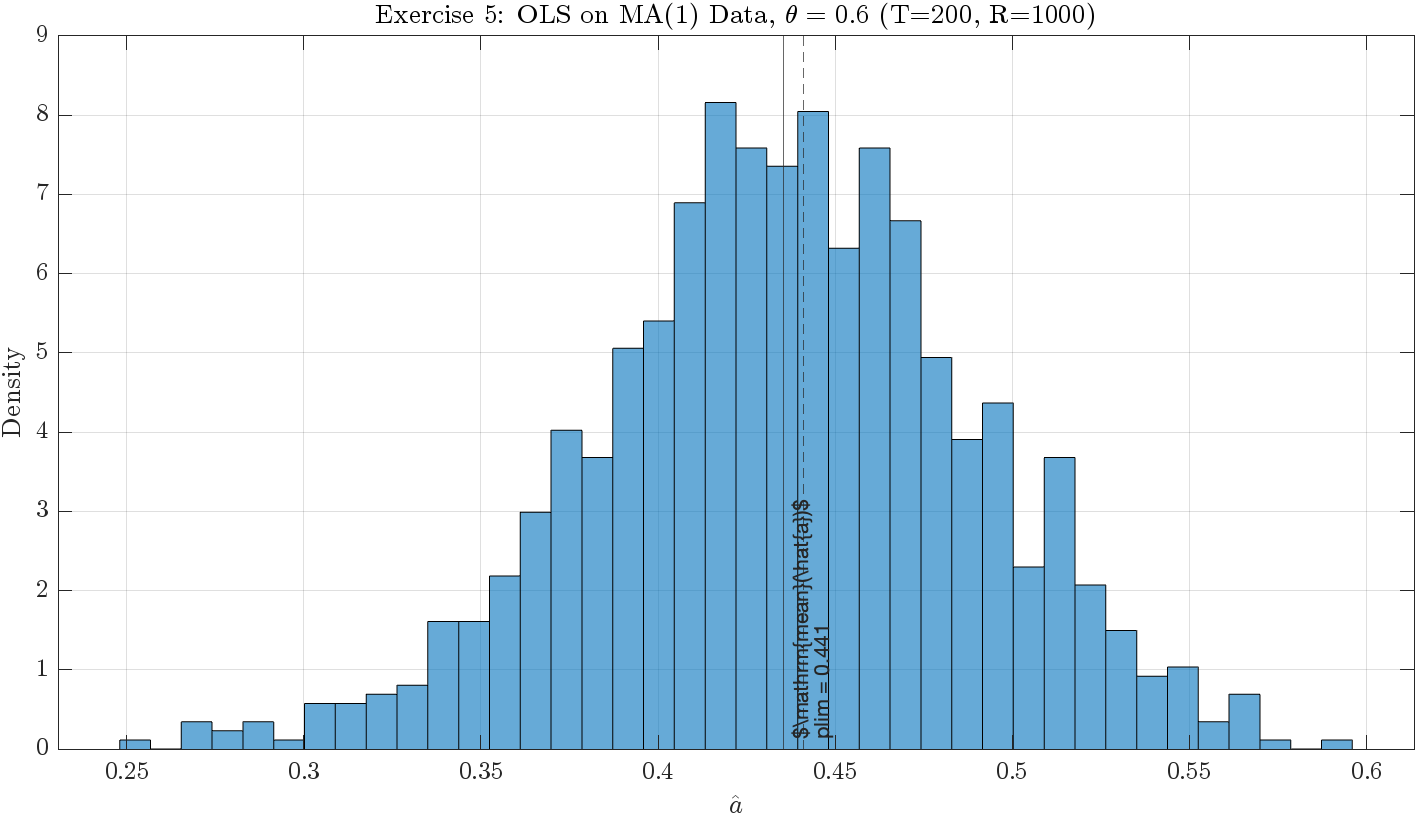
\includegraphics[width=\textwidth, trim=0cm 0cm 0cm 0.55cm, clip]{images/ex5_hist_T200.png}
                         \caption{\(T=200\)}
                         \label{fig:ex2_path_after_burnin}
                     \end{subfigure}
                     \hfill
                     \begin{subfigure}[b]{0.49\textwidth}
                         \centering
                         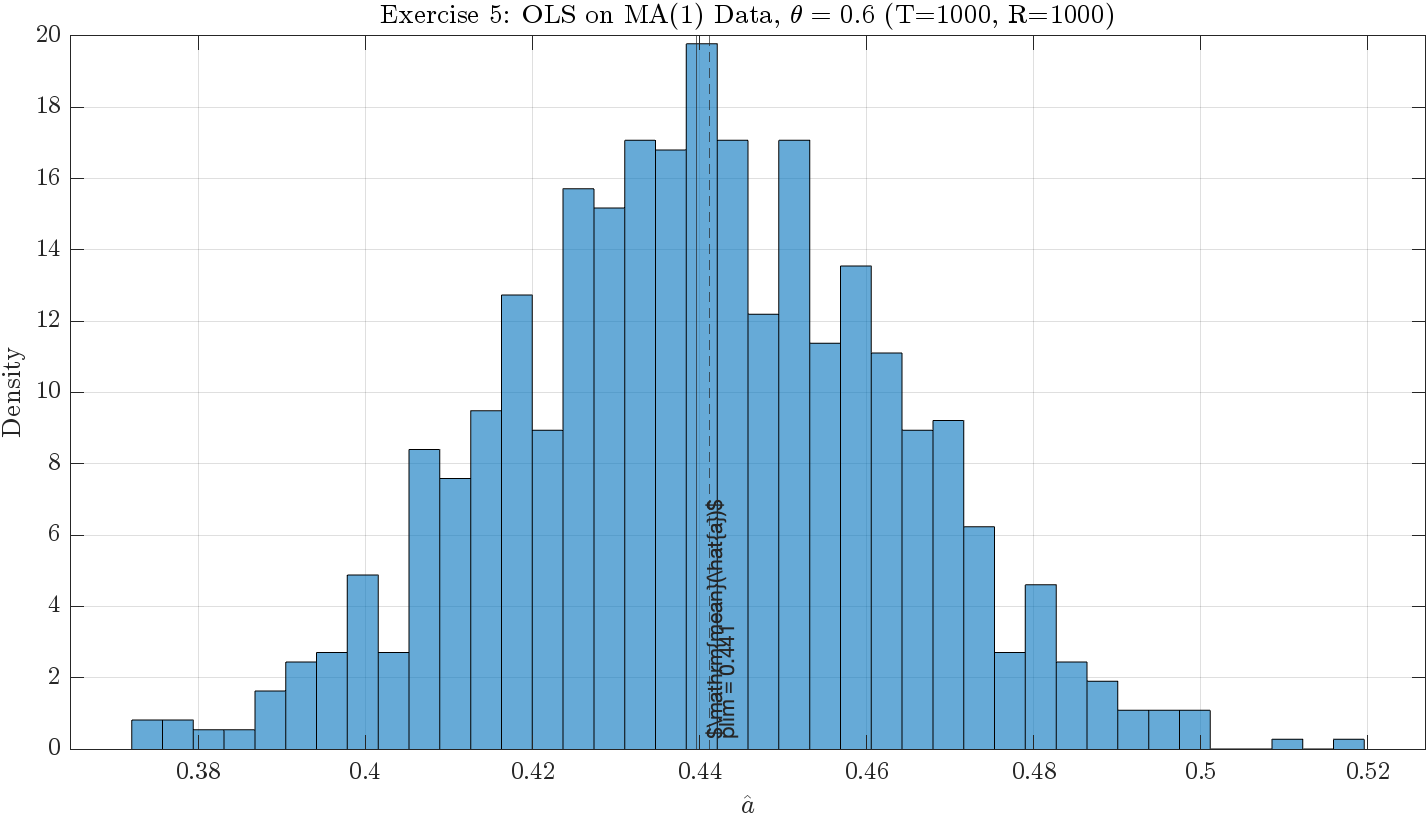
\includegraphics[width=\textwidth, trim=0cm 0cm 0cm 0.55cm, clip]{images/ex5_hist_T1000.png}
                         \caption{\(T=1000\)}
                         \label{fig:ex2_path_after_burnin}
                     \end{subfigure}
                    \label{fig:ex_1c}
                    \caption{Evolution of the distributions as the number of observations \(T\) increases.}
                \end{figure}

\newpage

        Focusing on the mean, we have:

        \[
        \begin{array}{r|cccc}
        T & 50 & 100 & 200 & 1000\\\hline
        \mathrm{mean}(\hat a) & 0.4345 & 0.4379 & 0.4354 & 0.4397
        \end{array}
        \]
        with empirical standard deviations approximately $(0.1065,\;0.0742,\;0.0535,\;0.0231)$, respectively.

        In light of these results, we can go back to the orignal question and discuss what happens to the \(\mathrm{mean}(\hat a) \):

        \begin{itemize}
            \item \textbf{Center (mean).} The Monte Carlo mean of $\hat a$ is close to $0.4412$ and drifts toward it as $T$ increases. Thus, the mean converges to the pseudo-true parameter $\rho(1)=\theta/(1+\theta^2)$, not to a structural AR(1) coefficient (there is no AR(1) here).
          
            \item \textbf{Spread (variance).} The dispersion of $\hat a$ shrinks with $T$ at the usual $\propto T^{-1/2}$ rate (histograms become more concentrated and more nearly normal around $0.4412$).
          
            \item \textbf{Interpretation.} Regressing $x_t$ on $x_{t-1}$ is estimating the \emph{best linear predictor} slope at lag 1. For MA(1) data, this equals the lag-1 autocorrelation. Hence, in large samples the OLS fit recovers $\rho(1)$.
        \end{itemize}

\begin{lstlisting}[language=matlab]
% Optional: plot mean(\hat{a}) across T for a compact summary figure
fh = figure('Position',[100 100 620 360]); grid on; hold on
plot(E5_summary.T, E5_summary.mean_a_hat, '-o', 'DisplayName','$\mathrm{mean}(\hat{a})$');
yline(plim_a, '--', 'DisplayName','theoretical plim');
xlabel('$T$'); ylabel('Mean of $\hat{a}$ across replications')
title('Exercise 5: Convergence of $\mathrm{mean}(\hat{a})$ with $T$', 'Interpreter','latex')
legend('Location','best')
exportFig(fh,'ex5_mean_vs_T.png');
\end{lstlisting}

        \begin{figure}[h]
            \centering
            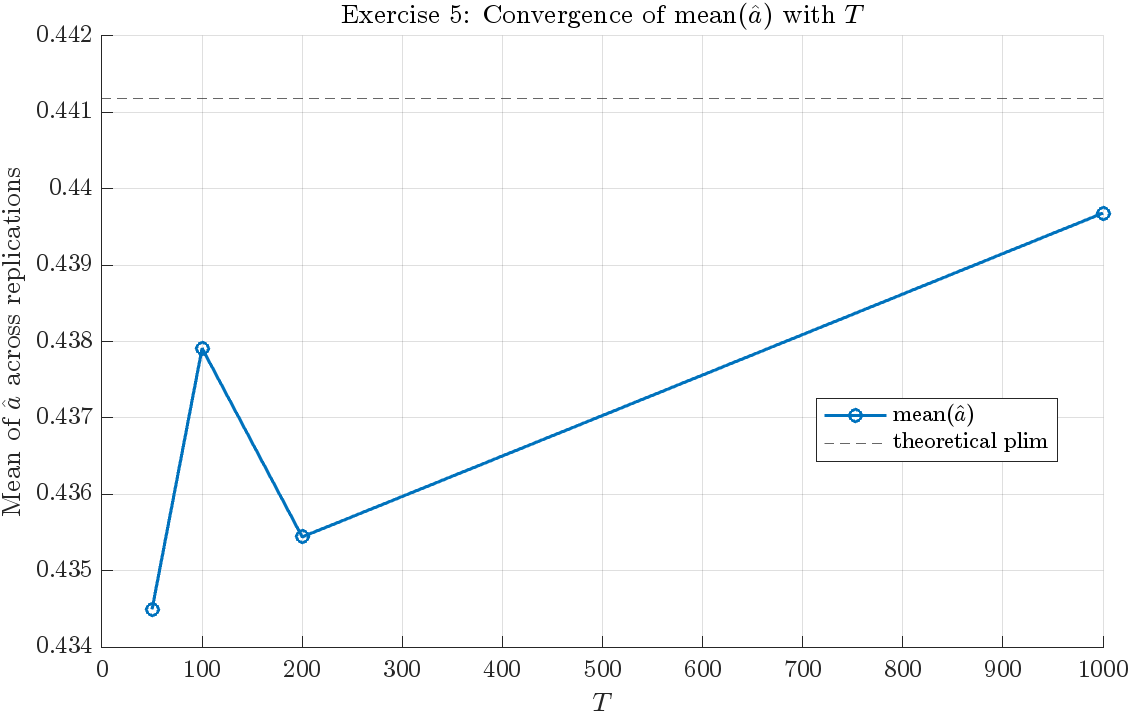
\includegraphics[width=0.65\linewidth]{images/ex5_mean_vs_T.png}
            \caption{Evolution of the mean\((\hat{a})\)}
            \label{fig:placeholder}
        \end{figure}
        
    \end{solution}

\section*{Question 6}
\setcounter{section}{6}

    Write a function that generates $T$ observations from an ARMA$(p,q)$ using the \texttt{for}-loop approach. The function must have the following inputs: 

    \begin{enumerate}[label=(\roman*)]
        \item the number of observations;
        \item the variance of the white noise $\varepsilon_t$
        \item the coefficients of the AR and MA polynomials or the roots of the AR and MA polynomials (hint: you may find the \texttt{poly} and \texttt{roots} functions useful);
    \end{enumerate}
    
    and as output the realizations of the ARMA$(p,q)$ and the white noise $\varepsilon_t$.

    \begin{solution}

        We tried to include all of the necessary informations and explanations directly in the function description down below.

\begin{lstlisting}[language=Matlab]
function [y, e] = arma_sim(T, sigma2, ar_in, ma_in, varargin) %#ok<DEFNU>
%ARMA_SIM Generate T observations from an ARMA(p,q) via for-loop.
%   y_t = mu + sum_{i=1}^p phi_i (y_{t-i} - mu) + e_t + sum_{j=1}^q theta_j e_{t-j}
%   with e_t ~ N(0, sigma2).
%
% Inputs (required):
%   T        -> number of observations to RETURN (after optional burn-in)
%   sigma2   -> variance of white noise e_t
%   ar_in    -> AR parameters: either coefficients [phi_1..phi_p] OR lag-roots [lambda_1..lambda_p]
%   ma_in    -> MA parameters: either coefficients [theta_1..theta_q] OR lag-roots [lambda_1..lambda_q]
%
% Name-Value pairs (optional):
%   'ParamType' -> 'coeffs' (default) or 'roots'.
%                 If 'roots', we interpret:
%                   A(L) = prod_{i=1}^p (1 - lambda_i L)  => 1 - phi_1 L - ... - phi_p L^p
%                   B(L) = prod_{j=1}^q (1 + lambda_j L)  => 1 + theta_1 L + ... + theta_q L^q
%                 Coefficients are then recovered from these lag polynomials.
%   'BurnIn'   -> number of burn-in observations to discard (default 500)
%   'Mu'       -> unconditional mean mu (default 0)
%
% Outputs:
%   y  -> T-by-1 vector of ARMA(p,q) observations
%   e  -> T-by-1 vector of shocks e_t used to generate y
%
% Notes:
%   * Stationarity (AR) / invertibility (MA) are the user's responsibility.
%   * We simulate with burn-in (default 500) from zero initial conditions.

    p = numel(ar_in); q = numel(ma_in);
    ip = inputParser; ip.KeepUnmatched = true;
    addParameter(ip,'ParamType','coeffs');
    addParameter(ip,'BurnIn',500);
    addParameter(ip,'Mu',0);
    parse(ip,varargin{:});

    paramType = validatestring(ip.Results.ParamType, {'coeffs','roots'});
    B = ip.Results.BurnIn; mu = ip.Results.Mu;

    % Determine phi and theta
    switch paramType
        case 'coeffs'
            phi = ar_in(:).';            % row
            theta = ma_in(:).';
        case 'roots'
            % Build lag polynomials and read off implied coefficients.
            if p>0
                poly_ar = 1; % A(L)
                for i=1:p
                    poly_ar = conv(poly_ar, [1, -ar_in(i)]); % (1 - lambda_i L)
                end
                phi = -poly_ar(2:end);   % A(L) = 1 - phi_1 L - ... - phi_p L^p
            else
                phi = [];
            end
            if q>0
                poly_ma = 1; % B(L)
                for j=1:q
                    poly_ma = conv(poly_ma, [1, ma_in(j)]); % (1 + lambda_j L)
                end
                theta = poly_ma(2:end); % B(L) = 1 + theta_1 L + ... + theta_q L^q
            else
                theta = [];
            end
    end

    % Sanity: warn if (approx) nonstationary / noninvertible
    if ~isempty(phi)
        A = [1, -phi(:).'];
        rr = roots(A);
        if any(abs(rr) <= 1)
            warning('AR polynomial has roots at or inside unit circle; process may be nonstationary.');
        end
    end
    if ~isempty(theta)
        Bpoly = [1, theta(:).'];
        rr = roots(Bpoly);
        if any(abs(rr) <= 1)
            warning('MA polynomial has roots at or inside unit circle; process may be noninvertible.');
        end
    end

    % Simulation with burn-in
    TT = T + B; p = numel(phi); q = numel(theta);
    e = sqrt(sigma2) * randn(TT,1);
    y = zeros(TT,1);
    if mu ~= 0
        % Work with deviations from mu for numerical stability
        x = zeros(TT,1);  % x_t = y_t - mu
        for t = 1:TT
            accAR = 0; accMA = 0;
            for i=1:p
                if t-i >= 1, accAR = accAR + phi(i) * x(t-i); end
            end
            for j=1:q
                if t-j >= 1, accMA = accMA + theta(j) * e(t-j); end
            end
            x(t) = accAR + e(t) + accMA;
        end
        y = x + mu;
    else
        for t = 1:TT
            accAR = 0; accMA = 0;
            for i=1:p
                if t-i >= 1, accAR = accAR + phi(i) * y(t-i); end
            end
            for j=1:q
                if t-j >= 1, accMA = accMA + theta(j) * e(t-j); end
            end
            y(t) = accAR + e(t) + accMA;
        end
    end

    % Drop burn-in
    y = y(B+1:end);
    e = e(B+1:end);
end
\end{lstlisting}
        
    \end{solution}



\end{document}
